\hypertarget{nuxe1stroje-pro-pruxe1ci-s-derivacuxed-v-ux10deskuxe9m-prostux159eduxed}{%
\chapter{Nástroje pro práci s~derivací v~českém
prostředí}\label{nuxe1stroje-pro-pruxe1ci-s-derivacuxed-v-ux10deskuxe9m-prostux159eduxed}}

Na základě onomaziologické teorie Miloše Dokulila (a~jeho následovníků)
vzniklo nemalé množství počítačových programů, prostřednictvím kterých
lze dosahovat různých výzkumných, edukačních či komerčních výsledků,
proto si v~první část této kapitoly popíšeme nejvýznamnější softwarové
nástroje, které se využívají pro práci s~derivací v~českém prostředí.
V~druhé části si pak hlouběji představíme derivační síť DeriNet, na níž je
postaveno řešení praktické části této bakalářské práce.

\hypertarget{pux159ehled-nuxe1strojux16f}{%
\section{Přehled nástrojů}\label{pux159ehled-nuxe1strojux16f}}

\hypertarget{morfio}{%
\subsection{Morfio}\label{morfio}}

Webová aplikace Morfio je jedním z~projektů Českého národního korpusu,
která „slouží k~odhadování rozsahu a~produktivity slovotvorných modelů
v~češtině na základě korpusových dat``. Jde tedy o~systém, který se snaží
ve zvoleném korpusu najít takové n-tice slov, které se shodují určitým
slovotvorným základem a~liší se specifickým slovotvorným formantem (těch
může být i~více, navíc je zde reflektována problematika hláskových
alternací.) Nástroj je tedy vhodný spíše jako výzkumná pomůcka než-li
jako prostředek ke tvorbě relevantních lingvistických výstupů, protože
při manipulaci s~korpusovými daty, jež nejsou nijak sémanticky
označkována, může docházet k~chybám například z~důvodu homonymie.
\parencite{cvrcek13}

\hypertarget{morfologickuxe9-analyzuxe1tory-ajka}{%
\subsection{Morfologické analyzátory
Ajka}\label{morfologickuxe9-analyzuxe1tory-ajka}}

Dalším nástrojem je morfologický analyzátor Ajka (vyvinutý na Masarykově
univerzitě), jehož hlavní složkou je analýza flektivní morfologie -- to
znamená, že obsahuje rozsáhlý systém vzorů spolu se sadami určitých
koncovek a~morfologických značek. Ve webovém rozhraní je možnost vstupní
text buď segmentovat na jednotlivé morfologické segmenty, analyzovat
z~pohledu určitého paradigmatu nebo vyhledat existující akcentovaný výraz
(například pro vstup \emph{blázen} je výstupem výraz \emph{blažen}).
Nástroj nicméně akcentuje i~složku derivační, a~to ve formě
hierarchického systému morfologických paradigmat, který slouží pro
zachycení všech úrovní derivační morfologie.~\parencite{ajka}

V~průběhu času vznikl z~potřeby efektivnějšího zpracování textu
z~morfologického analyzátoru Ajka nástroj Majka, který používá stejná
jazyková data, ale kompletně proměnil jejich formát a~stejně tak
algoritmus, který nad nimi operuje -- tak bylo docíleno větší rychlosti
zpracování.~\parencite{majka}

\hypertarget{deriv}{%
\subsection{Deriv}\label{deriv}}

Třetím relevantním softwarovým řešením zabývající se slovní derivací je
projekt Masarykovy univerzity Deriv, jenž je víceúčelovým nástrojem pro
automatické zpracování přirozeného jazyka s~primárním cílem testovat
možnosti automatické slovotvorné analýzy. Jeho webového rozhraní se
skládá ze dvou základních funkcí -- vyhledávání podle formálního zadání
a~kategorizace vyhledaných dat. Samotný Deriv je založený na
automatickém morfologickém analyzátoru Ajka (později Majka), v~rámci
kterého využívá jeho morfologický slovník kmenů a~vyhledává v~něm
prostřednictvím morfologických značek a~regulárních
výrazu\footnote{Nástroj využívá regulární výrazy programovacího jazyka Perl verze 5.10 a~novější.}.
Velkou výhodou aplikace je fakt, že jsou výsledky hledání propojeny
s~českými výkladovými slovníky (SSČ, SSJČ, PSJČ) a~s~některými českými
korpusy (konkrétně CzTenTen, SYN2000).~\parencite{deriv}

\hypertarget{derivancze}{%
\subsection{Derivancze}\label{derivancze}}

Předposledním rozebíraným nástrojem je derivační analyzátor Derivancze,
který analyzuje slovotvorné vztahy mezi slovy. Využívá veřejně přístupná
data derivační sítě DeriNet, ale na rozdíl od ní pracuje pouze se
sémantickými vztahy, to znamená, že pokud se liší formální a~významový
aspekt derivačního vztahu, tak je vyžadováno explicitní označkovaní,
díky kterému pak dochází ke konzistenci napříč daty. Nástroj využívá
sedmnácti značek označující typ sémantického vztahu -- může jít
například o~značku \emph{k1ag}, která označuje vztah odvození verba
směrem k~činitelskému jménu. Nicméně tento přístup vytváří určité
problémy, nastroj je problematické použit v~rámci větších
sofistikovanějších aplikací (například automatické generování textu),
protože by bylo zapotřebí dodat více informací o~typech jednotlivých
slovotvorných vztahů.~\parencite{derivancze}

\hypertarget{derivaux10dnuxed-suxedux165-derinet}{%
\section{Derivační síť
DeriNet}\label{derivaux10dnuxed-suxedux165-derinet}}

Řešení praktické části této bakalářské je postaveno na derivační síti
DeriNet, proto si tento nástroj v~následující podkapitole hlouběji
charakterizujeme a~popíšeme základní přístupy, jak s~ním lze pracovat.

Derivační síť DeriNet si lze představit jako elektronickou databázi
českých autosémantik (tedy primárně substantiv, adjektiv, verb
a~adverbií), která jsou vzájemně propojena takovými odkazy, jež odpovídají
slovotvornému vztahu derivace mezi slovem základovým a~odvozeným. Tento
systém odkazů si lze tak modelovat prostřednictvím orientovaného grafu,
jehož uzly jsou jednotlivá lemmata (základní slovní tvary) a~hrany pak
spolu s~jejich orientací reprezentují určitý odvozovací proces. Jelikož
má v~této derivační síti každé odvozené slovo odkaz pouze na jedno slovo
základové, lze si tak jednotlivé slovotvorná hnízda (čeledě) představit
jako stromový graf, jehož kořenem je ideálně slovo značkové, tedy takový
výraz, který není nijak motivován.~\parencite{derinet-cz}

Před samotným vznikem tohoto projektu bylo řešeno několik lingvistických
skutečností, které ovlivnily výslednou podobu DeriNetu -- primárně šlo
o~problematiku výběru původních lexémů, zde existovaly dvě varianty, buď
využít již existujících jazykových dat z~korpusů nebo poloautomaticky
generovat daná lemmata, zde bylo rozhodnuto držet se úzu a~extrahovat
lexémy z~korpusu (konkrétně šlo o~korpus řady SYN a~bylo vybráno
přibližně dvě stě šedesát tisíc lemmat). Druhou otázkou bylo, jaký typ
slovotvorného vztahu by měl být v~lexikální síti reflektován, v~tomto
případě byla vybrána derivace z~důvodu svého dominantního postavení
v~české slovotvorbě, nicméně je do budoucna plánováno popsat i~slovotvorné
vztahy týkající se skládání slov, to by ale kompletně pozměnilo
architekturu sítě, kde má každé základové slovo právě jen jeden odkaz na
určitý derivát.~\parencite{sevcikova14}

Pro tvorbu samotné derivační sítě, resp. jednotlivých derivačních vztahů
bylo zapotřebí identifikovat dvojice slov základových a~odvozených --
toho bylo docíleno poloautomatickou metodou, šlo tedy nejprve
o~automatizovaný výběr takových dvojic lemmat, v~rámci kterých měla obě
slova dostatečně dlouhý společný počáteční podřetězec a~zároveň se
lišila specifickým koncovým podřetězcem. Ze čtyř set
nejfrekventovanějších pak bylo ručně vyextrahováno osmnáct dvojic, které
odpovídají popisovaným derivačním vztahům v~české slovní zásobě,
u~těchto dvojic byl taktéž určen směr derivace (typicky bylo za základové
slovo považováno to, které mělo kratší základové lemma).
\parencite{derinet-cz}

Dalším způsobem, pomocí kterého šlo určovat derivační vztahy, byla
extrakce informací z~morfologického slovníku MorFlex CZ -- ten obsahuje
sto dvacet milionů trojic tvořených lemmatem, morfologickou značkou
a~slovním tvarem, příkladem může být trojice ‒ \emph{žížnivý\_,n};
\texttt{AAFS6-\/-\/-\/-3N-\/-\/-\/-}; \emph{nejnežížnivější}.
\parencite{morflex}

Jednotlivá lemmata mohou taktéž obsahovat dodatečnou derivační
a~sémantickou informaci, právě tak slovník řeší například problematiku
lexikální homonymie, kdy jsou homonymní lemmata označena specifickým
číselným identifikátorem (např. \emph{podle-1} ve významu adverbia
a~\emph{podle-2} jako prepopozice). Derivační informace je ve slovníku
reprezentována prostřednictvím technického sufixu, který je uložen
u~daného lemmatu (např. u~základního tvaru \emph{žíznitelný\_\^{}(}4)* je
derivační informace uložena v~závorce a~vyplývá z~ní, že je slovo
\emph{žíznitelný} odvozeno od slova o~čtyři znaky kratšího, tedy od
slova \emph{žíznit}). Díky datům ze slovníku MorfFlex CZ byl počet
lemmat v~DeriNetu přibližně ztrojnásoben a~zároveň doplněn o~velké
množství derivačních vztahů.~\parencite{sevcikova16}

\begin{figure}[ht]   
    \centering
    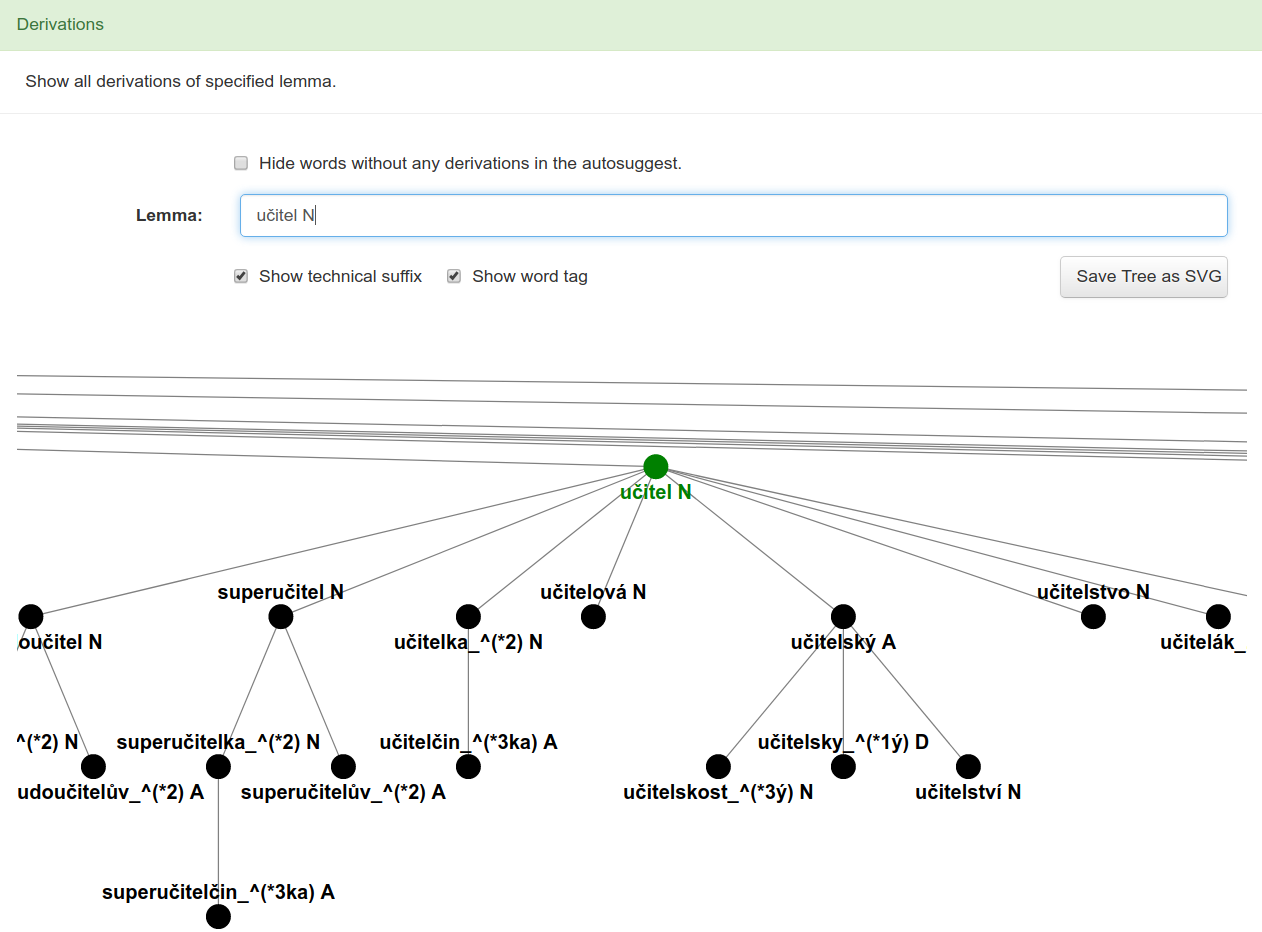
\includegraphics[width=.9\textwidth]{derinet-1}  
    \caption{Výsledný derivační strom v~prohlížeči DeriNet Viewer~\parencite{derinet}}
    \label{derinet-1}
 \end{figure}

Aktuální verze derivační sítě DeriNet (1.7) obsahuje přibližně jeden
milion lemmat a~je dostupná skrze dvě webová uživatelská rozhraní.
Jedním z~nich je prohlížeč DeriNet
Viewer\footnote{Autor je Milan Straka -- http://ufal.mff.cuni.cz/derinet/derinet-viewer},
jehož základní funkcí je zobrazení derivačního stromu pro zadané lemma
(srov. obr. \ref{derinet-1}), případně lze vyhledané výsledky roztřídit
podle zvolených charakteristik. Druhý nástroj je DeriNet
Search\footnote{Autor je Jonáš Vidra -- http://ufal.mff.cuni.cz/derinet/search.},
který nabízí vyhledávání ve vlastním dotazovacím jazyce, to znamená, že
si je tak uživatel schopen podle svých vlastních kritérii specifikovat
omezení pro tvar vyhledaného derivačního stromu. Například dotaz
\texttt{{[}pos="V"{]}\ ({[}pos="N"\ lemma="tel\$"{]},\ {[}pos="N"\ lemma="ce\$"{]})}
vyhledá takové derivační stromy, ve kterých je od verba přímo odvozeno
jednak substantivum končící na sufix \emph{-tel}, tak substantivum končící příponou \emph{-ce} (viz obr. \ref{derinet-2}).~\parencite{derinet-cz}

\begin{figure}[ht]   
    \centering
    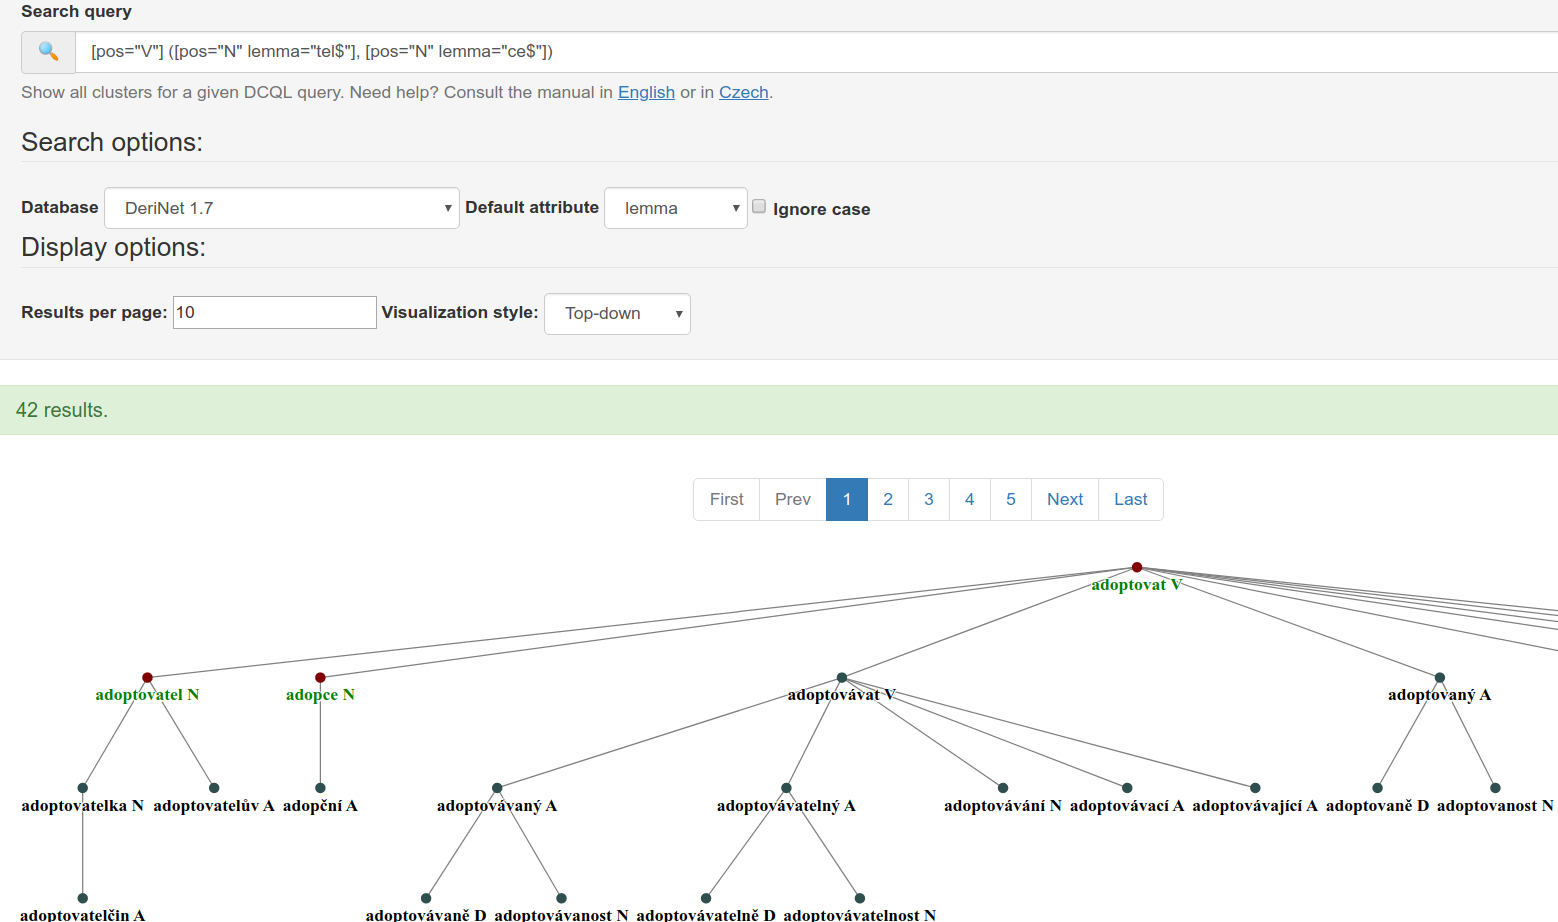
\includegraphics[width=.9\textwidth]{derinet-2}  
    \caption{Výsledek vyhledávacího dotazu ve vyhledávači DeriNet Search~\parencite{derinet}}
    \label{derinet-2}
 \end{figure}

Další možnost jak pracovat s~databází DeriNet je prostřednictvím
jednoduchého datového formátu TSV (anglicky \emph{Tab-Separated Values},
jde o~textovou reprezentaci tabulkových dat, které jsou od sebe odděleny
tabulátorem), jenž je zpřístupněn k~volnému stažení pod licencí Creative
Commons Attribution-NonCommercial-ShareAlike 3.0
License\footnote{https://creativecommons.org/licenses/by-nc-sa/3.0/}.
U~tohoto přístupu se již počítá se základními programátorskými
dovednostmi, protože takto strukturovaná data primárně slouží jako vstup
pro určitý software.~\parencite{derinet-cz}

Každá položka v~tomto souboru obsahuje několik atributů, jde o~vlastní
identifikační číslo, lemma, derivační informaci přejatou
z~morfologického slovníku MorFlex CZ, značku slovního druhu a~u~slov
derivovaných identifikační číslo slova základového -- tím je jednoznačně
vyznačen derivační vztah (viz obr. \ref{derinet-3}). Právě tento formát
DeriNetu je použitý jako základ pro tvorbu samotného derivačního
slovníku v~rámci praktické části této práce.

\begin{figure}[ht]   
    \centering
    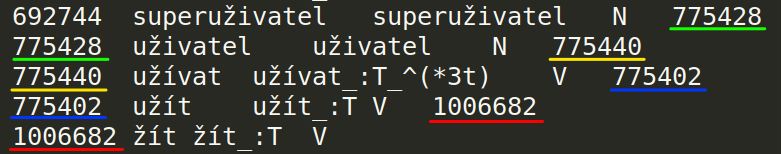
\includegraphics[width=.9\textwidth]{derinet-3}  
    \caption{Formát TSV s~vyznačenými identifikačními čísly, které společně vytvářejí derivační řetězec~\parencite{derinet}}
    \label{derinet-3}
 \end{figure}
